
\section{Graph Programs}
\label{sec:graph-programs}

This paper focusses on GP~2, a successor to the graph programming language GP \cite{Plump09a,Plump12a}.
GP is a domain-specific language which aims to support formal reasoning on graph programs (see \cite{Poskitt-Plump12a} for a Hoare-logic approach to verifying GP programs). We give a brief introduction to GP~2, mainly by example. The definition of the language, including a formal operational semantics, can be found in \cite{Plump12a}. 

A graph program consists of declarations of conditional graph transformation rules and macros, and exactly one main command sequence. Graphs are directed and may contain  loops and parallel edges. The rules operate on a \emph{host graph}\/ (or input graph) whose nodes and edges may be labelled.

Labels are of type \texttt{int} (for integers), \texttt{char} (for characters), \texttt{string} (for character strings), \texttt{atom} or \texttt{list}, where \texttt{atom} is the union of \texttt{int}, \texttt{char} and \texttt{string}. Atoms are considered as lists of length one, hence integers and strings are also lists. Given lists $\mtt{x}$ and $\mtt{y}$, their concatenation is written \texttt{x:y} (not to be confused with the list-cons operator in Haskell). 
We proceed by discussing two example programs.

\begin{example}[Transitive Closure]
The principal programming constructs in GP~2 are conditional graph-transformation rules labelled with expressions. The program in Figure \ref{fig:transitive-closure} applies the single rule \ttt{link} \emph{as long possible} to a host graph. In general, any subprogram can be iterated by applying \ttt{!} as a postfix operator.

\begin{figure}[htb]
\begin{center}
 \input{Programs/trans_closure.prog}
\end{center}
%\vspace{-.5\baselineskip}
\caption{Program for transitive closure}\label{fig:transitive-closure}
\end{figure}

Applying \ttt{link} amounts to non-deterministically selecting a subgraph of the host graph that matches \ttt{link}'s left graph, and adding to it an edge from node 1 to node 3 provided there is no such edge (with any label). The application condition ensures that the program terminates and extends the host graph with a minimal number of edges.

A graph is \emph{transitive} if for each directed path from a node $v$ to another node $v'$, there is an edge from $v$ to $v'$.  Given any graph $G$, the program in Figure \ref{fig:transitive-closure} produces the smallest transitive graph that results from adding unlabelled edges to $G$.\footnote{``Unlabelled'' edges are actually labelled with the empty list.} This graph is unique up to isomorphism and requires at most $n^2$ applications of \ttt{link}, where $n$\/ is the number of nodes in $G$. \qed
\end{example}
  

\begin{example}[Vertex Colouring]
The program in Figure \ref{fig:vertex-colouring} assigns a \emph{colour}\/ to each node of the host graph, such that non-loop edges have differently coloured endpoints. Positive integers are used as colours because, in general, an unbounded number of colours is needed. The program replaces each node label $l$\/ with $l{:}i$, where $i$\/ is the node's colour. In addition, the rule \ttt{init} shades nodes to prevent repeated application to the same node.
% (Nodes can be graphically \emph{marked}\/ by drawing them shaded or in one of the colours red, green or blue.)

\begin{figure}[htb]
\begin{center}
 \input{Programs/vertex-colouring.prog}
\end{center}
%\vspace{-.5\baselineskip}
\caption{Program for vertex colouring}\label{fig:vertex-colouring}
\end{figure}

Rule \ttt{inc} is applied to the host graph as long as there are edges with identically coloured endpoints. It can can be shown that this terminates after at most $n^2$ rule applications, where $n$\/ is the number of nodes. In contrast to the previous example program, \emph{different graphs may result}\/ from this process. In particular, there is no guarantee that the number of colours produced is minimal. For instance, Figure \ref{fig:colour_results} shows two different colourings produced for the same host graph.
\qed
\end{example}

\begin{figure}[htb]
\begin{center}
 \input{Graphs/colour_results.graph}
\end{center}
%\vspace{-.5\baselineskip}
\caption{Different results from vertex colouring}\label{fig:colour_results}
\end{figure}

\vspace{.5\baselineskip}
\noindent
\emph{Other program constructs.}
A GP~2 command not used in the example programs is a rule set $\mtt{\{}r_1,\dots,r_n\mtt{\}}$. This command \emph{non-deterministically} applies any of the rules to the current host graph. The application \emph{fails}\/ if none of the left-hand graphs in the rules matches a subgraph. Matches must be injective and are only valid if they do not result in \emph{dangling edges}.

Another construct not yet discussed is the branching command \ttt{if} $C$ \ttt{then} $P$ \ttt{else} $Q$, where $C$, $P$ and $Q$ are arbitrary command sequences. This is executed on a host graph $G$ by first executing $C$ on a copy of $G$. If $C$ succeeds, $P$\/ is executed on the original graph $G$; otherwise, $Q$ is executed on $G$. The command \ttt{try} $C$ \ttt{then} $P$ \ttt{else} $Q$ has a similar effect, except that $P$\/ is executed on the graph resulting from $C$'s execution. 

\section{Benchmark Programs}
\label{sec:benchmark}
 
Besides the programs for transitive closure and vertex colouring, we select four more programs for benchmarking.


\subsection{Shortest distances}

\begin{tabular}{lp{10.5cm}}
\ul{Input:} & A graph $G$ with a unique grey node $s$. All edge labels are non-negative integers. \\
\ul{Output:} & The graph obtained from $G$ by marking grey each node reachable from $s$ and replacing its label $l$\/ with $l{:}d$, where $d$\/ is the shortest distance from $s$. (A distance is the sum of the edge labels of a directed path.)
\end{tabular}
  
\begin{center}
\input{Programs/distances.prog}
\end{center}

\ul{Notes}
\begin{enumerate}
\setlength{\itemsep}{-.5ex}
\item The output is unique up to isomorphism.
\item The input requirement can be relaxed by allowing negative edge labels but forbidding directed cycles with a negative distance.
\end{enumerate}


\subsection{Recognising acyclic graphs}
\label{sec:acyclic}

\begin{tabular}{lp{10.5cm}}
\ul{Input:} & Any graph $G$. \\
\ul{Output:} & Graph $G$ if it is acyclic, otherwise the program fails.
\end{tabular}
  
\begin{center}
\input{Programs/acyclic.prog}
\end{center}


\subsection{Rooted 2-colouring}

\begin{tabular}{lp{10.5cm}}
\ul{Input:} & A non-empty, single-rooted, connected graph $G$ with atomic labels. \\
\ul{Output:} & If $G$\/ is 2-colourable, then the output is obtained from $G$\/ by marking each node with either red or blue. The source and target of each non-loop edge have different colours.\\
& If $G$\/ is not 2-colourable, then the output is $G$.
\end{tabular}

\begin{center}
\begin{tikzpicture} [scale=0.7,align=center,auto,inner sep=2mm,arrowin,arrowout,font=\ttfamily]
\node at (4.75,3.8) {main = try (init; colouring; unshaded)};
\node at (6.75,3.2) {colouring = ((colour; if invalid then stop)!; back)!};
\node at (4,2.6) {colour = \{colour-blue,colour-red\}};
\node at (4.45,2) {invalid = \{joined-reds,joined-blues\}};

%init
\node at (0,0)[root,label=below:\scriptsize{1}]{x};
\node at (1.2,0){$\Rightarrow$};
\node at (1,0)[above=5mm] {init(x:atom)};
\node at (2.4,0)[root,fill=red!75,label=below:\scriptsize{1}]{x};

%stop
\begin{scope}[yshift=-3cm]
\node (l1) at (0,0)[root,label=below:\scriptsize{1}]{x};
\node at (1.2,0){$\Rightarrow$};
\node at (1,0)[above=5mm] {stop(x:atom)};
\node (r1) at (2.4,0)[root,fill=black!20,label=below:\scriptsize{1}]{x};
\end{scope}

%unshaded
\begin{scope}[yshift=-6cm]
\node (l1) at (0,0)[root,label=below:\scriptsize{1}]{x};
\node at (1.2,0){$\Rightarrow$};
\node at (1.5,0)[above=5mm] {unshaded(x:atom)};
\node (r1) at (2.4,0)[root,label=below:\scriptsize{1}]{x};
\end{scope}

%colour-red
\begin{scope}[xshift=5.5cm]
\node (l1) at (0,0)[root,fill=red!75,label=below:\scriptsize{1}]{x};
\node (l2) at (2.9,0)[inner sep = 2mm,circle,draw,label=below:\scriptsize{2}]{y}
   edge [-] node[above]{a} (l1);
\node at (4.1,0){$\Rightarrow$};
\node at (3.2,0)[above=5mm] {colour-red(a:list; x,y:atom)};
\node (r1) at (5.3,0)[circle,draw,fill=red!75,label=below:\scriptsize{1}]{x};
\node (r2) at (8.2,0)[root,fill=blue!60,label=below:\scriptsize{2}]{y}
  edge [-,dashed] node[above]{a} (r1);  
\end{scope}

%joined-reds
\begin{scope}[xshift=5.5cm,yshift=-3cm]
\node (l1) at (0,0)[root,fill=red!75,label=below:\scriptsize{1}]{x};
\node (l2) at (2.9,0)[circle,draw,fill=red!75,label=below:\scriptsize{2}]{y}
  edge [-] node[above]{a} (l1);
\node at (4.1,0){$\Rightarrow$};
\node at (3.3,0)[above=5mm] {joined-reds(a:list; x,y:atom)};
\node (r1) at (5.3,0)[root,fill=red!75,label=below:\scriptsize{1}]{x};
\node (r2) at (8.2,0)[circle,draw,fill=red!75,label=below:\scriptsize{2}]{y}
  edge [-] node[above]{a} (r1);
\end{scope}

%back
\begin{scope}[xshift=5.5cm,yshift=-6cm]
\node (l1) at (0,0)[root,fill=red!75,label=below:\scriptsize{1}]{x};
\node (l2) at (2.9,0)[circle,draw,fill=blue!60,label=below:\scriptsize{2}]{y}
  edge [-,dashed] node[above]{a} (l1);  
\node at (4.1,0){$\Rightarrow$};
\node at (2.4,0)[above=5mm] {back(a:list; x,y:atom)};
\node (r1) at (5.3,0)[circle,draw,fill=red!75,label=below:\scriptsize{1}]{x};
\node (r2) at (8.2,0)[root,fill=blue!60,label=below:\scriptsize{2}]{y}
  edge [-] node[above]{a} (r1);
\end{scope}

\draw (-1.2,4.4) rectangle (15.2,-7.5);

\end{tikzpicture}

\end{center}

\ul{Notes}
\begin{enumerate}
\setlength{\itemsep}{-.5ex}
\item The edges in the rules \ttt{colour}, \ttt{joined-reds} and \ttt{back} are \emph{bidirectional}. They matches host graph edges in either direction.
\end{enumerate}


\subsection{Generating Sierpinski triangles}

\begin{tabular}{lp{10.5cm}}
\ul{Input:} & A single node labelled with a non-negative integer $n$. \\
\ul{Output:} & The Sierpinski triangle of generation $n$.
\end{tabular}
  
\begin{center}
\input{Programs/sierpinski.prog}
\end{center}

\ul{Notes}
\begin{enumerate}
\setlength{\itemsep}{-.5ex}
\item The next page shows an example of a Sierpinski triangle.
\item The derivation length and the output size are exponential in $n$.
\end{enumerate}

\begin{figure}[htb]
 \begin{center}
  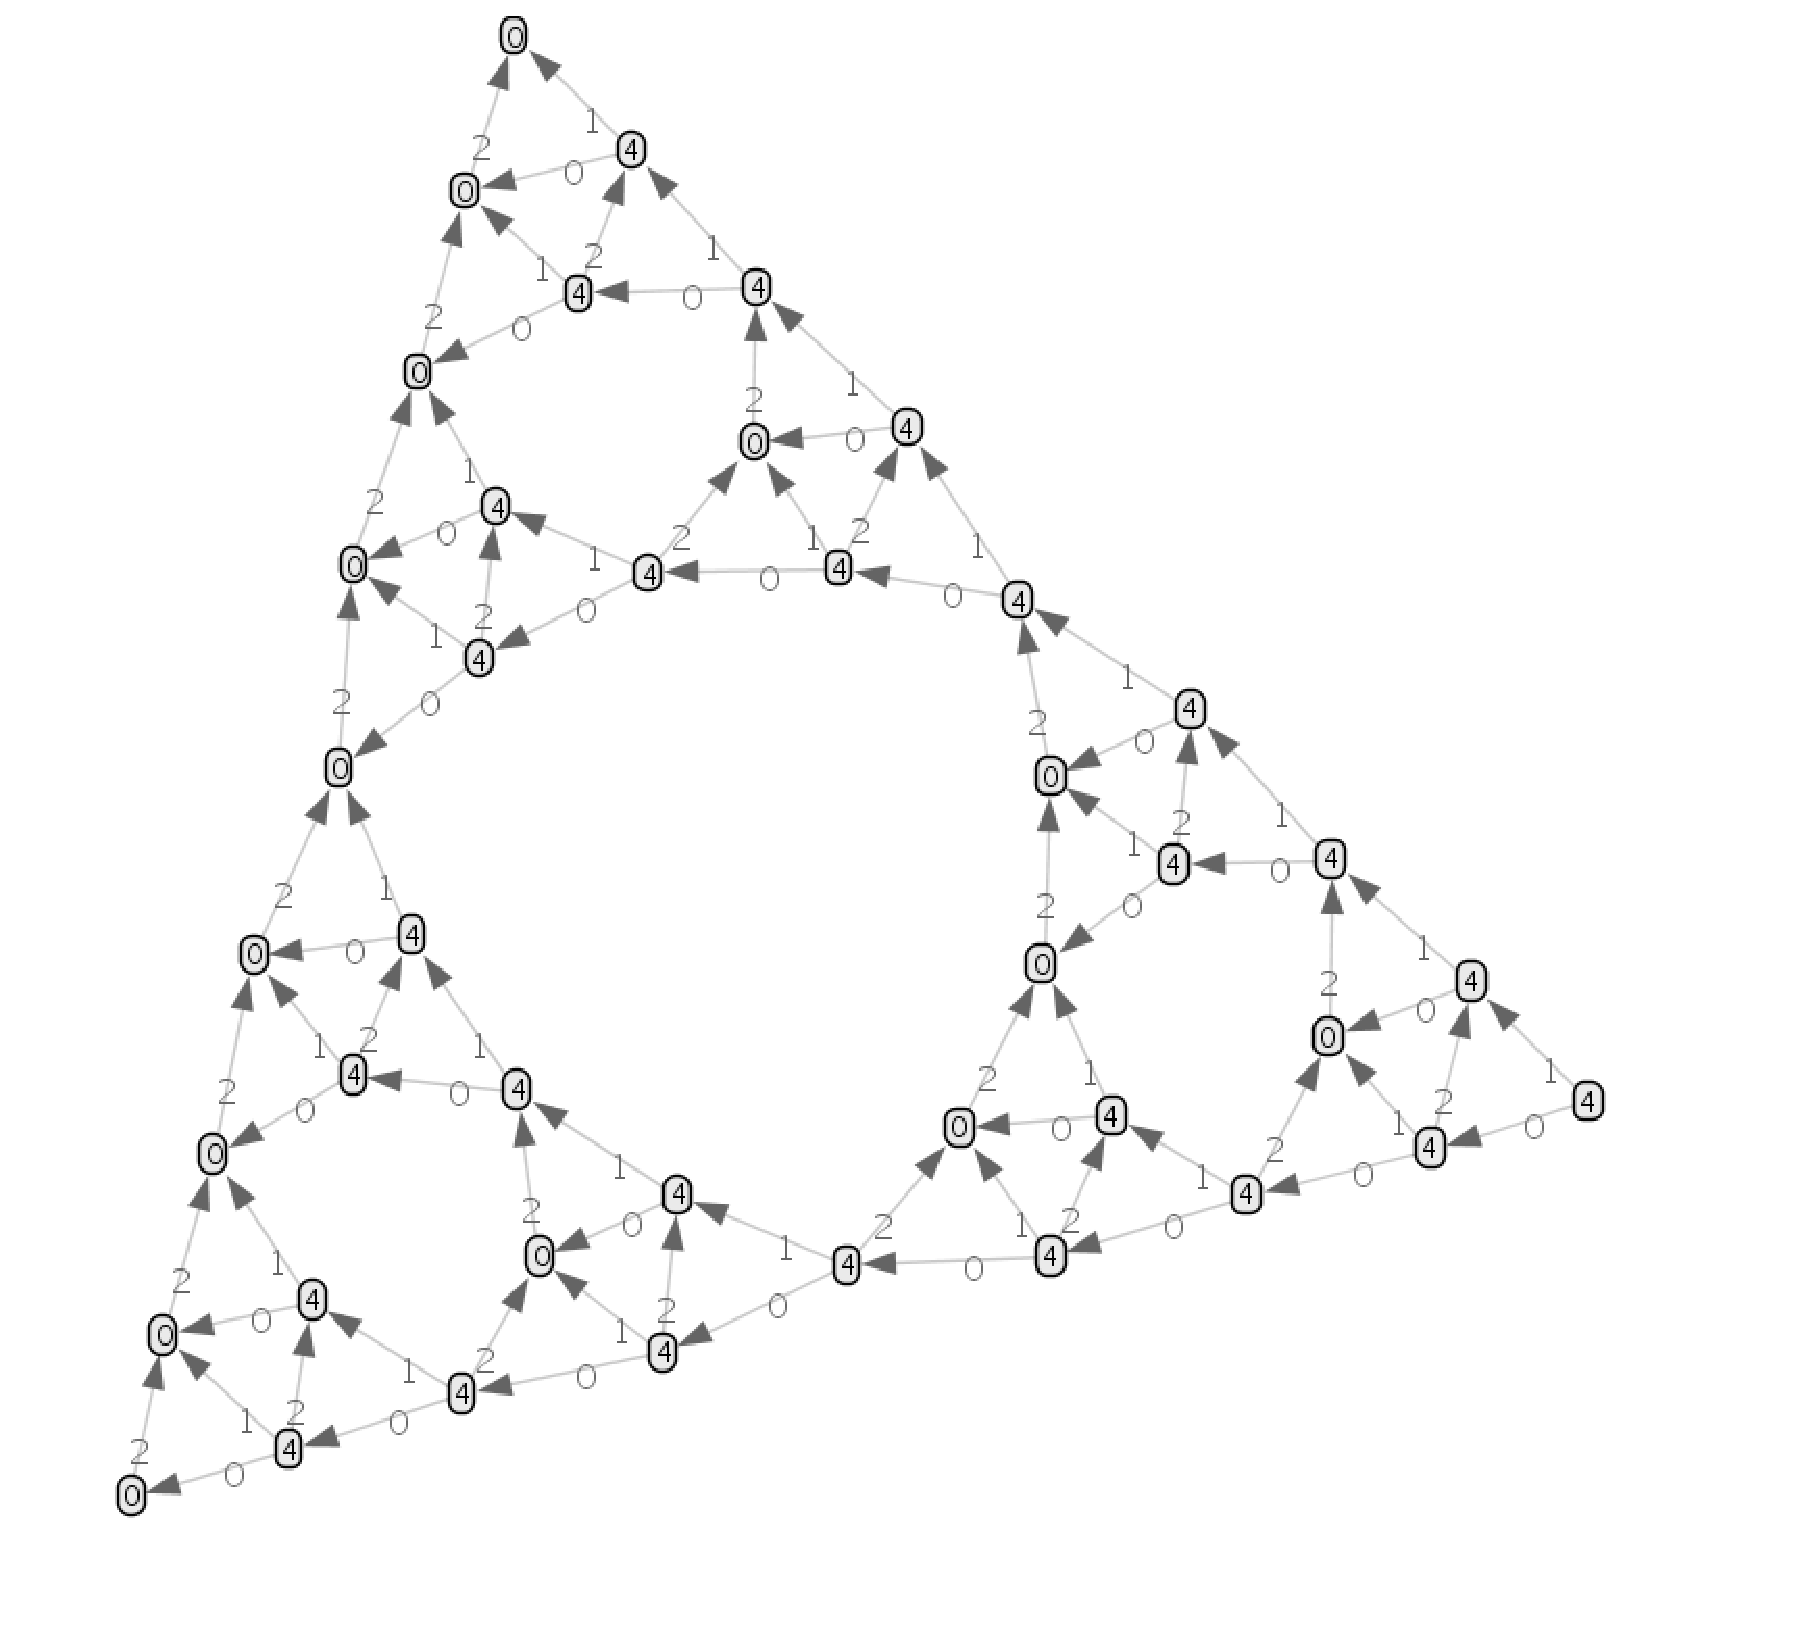
\includegraphics[scale=.4,angle=-15]{sierpinski-3.eps}
 \end{center}
\vspace*{-2.5cm}
\caption{Third generation Sierpinski triangle \label{fig:sierpinski}}
\end{figure}




\section{The implementation}


\subsection{Data structures}

The reference interpreter uses a trivial implementation of an extensible array library, written initially without concern for performance issues, but encapsulated in such a way as to be replaceable with a more efficient library later if required. Specifically, a graph is represented as a pair of extensible arrays: one for the nodes and one for the edges.

\subsection{Program environment}

\subsection{Graph matching}

The graph matcher constructs a list of GraphMorphisms, where a GraphMorphism is a data structure containing the program environment, namely the variable-value assignments; a mapping between the NodeIds in the LHS of the rule graph and the corresponding NodeIds in the host graph; and a similar list of EdgeId mappings. Morphisms are generated by first constructing the set of all possible NodeMorphisms, then augmenting each node morphism with appropriate edge mappings. A NodeMorphism is a GraphMorphism without a list of EdgeId mappings.


The node matching algorithm takes as input the LHS L and the host graph G. It works as follows:

\begin{enumerate}
	\item Count the number of nodes k in L.
	\item Generate all sets of size k containing nodes from G.
	\item Iterate through the sets from step 2, comparing node labels in L to labels in G. Keep the sets in which node labels correspond for all pairs of nodes.
\end{enumerate}

It is clear that the complexity of this algorithm increases rapidly with both the size of L and the size of G. This is a naive matching strategy that would not be appropriate if performance were a consideration. In this case, where correctness is a greater concern, the simplicity of this algorithm is of benefit by making the source code easier to reason about.


The edge-matching algorithm takes as input the LHS L, the host graph G and a node morphisms NM. It works as follows:


\begin{enumerate}
	\item Get the source and target of each edge in L.
	\item Using NM, translate each source and target pair to the corresponding pair of host graph nodes.
	\item For each pair of host graph nodes (source, target), get the set of edges in G from source to target.
	\item Associate each edge in L with its set of candidate edge matches found in step 3.
	\item For all edges in L, test their label against the labels of each of its candidate matches. If the host label matches the LHS label (possibly with a variable-value assignment), add the assignment to the environment and add the edge match to the morphism. Otherwise, do nothing.
\end{enumerate}


Since it only generates edge sets that conform to the structural requirements of a graph morphism, it is more sophisticated than the node matching algorithm. The edge-matching algorithm has a smooth implementation due to features of Haskell. The first four steps are achieved with maps, ensuring that each LHS-edge is paired up with the correct set of host-edges.


\subsection{The dangling condition}

In the double-pushout framework of graph transformation, on which GP 2 is based, a rule may not be applicable for a particular match as applying the rule could leave an edge without a source or target. The dangling condition forbids this: it requires that all host edges not deleted by the rule are not incident to nodes deleted by the role.


\subsection{Isomorphism checking}

Producing all possible output graphs leads to the issue that many of the results may be isomorphic. To simplify analysis of the results, we implemented a basic isomorphism checker, so that our program completes with a set of all possible distinct output graphs, plus a count of the number of isomorphic variants of each graph that were seen.


\subsection{Rooted graphs}

Lessons learned from the implementation of the original GP language led to the addition of support for root nodes to GP2. A node carries a simple binary flag indicating whether it is a root node or not. A root node in a rule graph can only match a root node in the host graph, and then only if all other normal matching conditions are met, eliminating a large number of possible subgraph matches with only an inexpensive boolean test. Whereas a non-root node in the rule graph may match a node irrespective of its root-node status.


Even in the reference interpreter, addition of a root node can result in a significant performance gain of TODO.

